  \documentclass[utf8]{beamer}
\usepackage[spanish]{babel}
\usetheme{Warsaw}
\setbeamertemplate{headline}{}
\usefonttheme{serif}
%\usepackage{times}
\usepackage{helvet}
\usepackage{ragged2e}
\justifying

  \usepackage{physics}
  \usepackage{amsmath}
  \usepackage{amssymb}
  \usepackage{mathrsfs}
  \usepackage{graphicx}
  \usepackage{float}
  \usepackage{siunitx}
  \usepackage{subfigure}
  \usepackage{enumerate}
  \usepackage{comment}
  \usepackage{hyperref}

\title{Proyecto de Modelado Matemático I: \\ Visualización 3D en VisIt}
\author{Paula Camila Wandurraga Sanabria}
\institute{Maestría en Matemática Aplicada \\ Grupo de Investigación en Relatividad y Gravitación \\ Universidad Industrial de Santander}
\date{}

\begin{document}
	\begin{frame}
		\titlepage
	\end{frame}

%\begin{block}{Observation 1}
%Simmons Hall is composed of metal and concrete.
%\end{block}
%\begin{exampleblock}{Observation 2}
%Simmons Dormitory is composed of brick.
%\end{exampleblock}
%\begin{alertblock}{Conclusion}
%Simmons Hall $\not=$ Simmons Dormitory.
%\end{alertblock}

%%%%%%%%%%%%%%%%%%%%%%%%%%%%%%%%%%%%%%%%%%%%%%%%%%%%%%%%%%%%%%%%%%


\begin{frame}{Planteamiento del problema}
	\includegraphics[width=5.5cm]{figs/pic1.png}
	\includegraphics[width=5.5cm]{figs/pic2.png}
\end{frame}

\begin{frame}{}
	\centering
	\includegraphics[width=11cm]{figs/pic3.png}
\end{frame}

\begin{frame}{VisIt}
	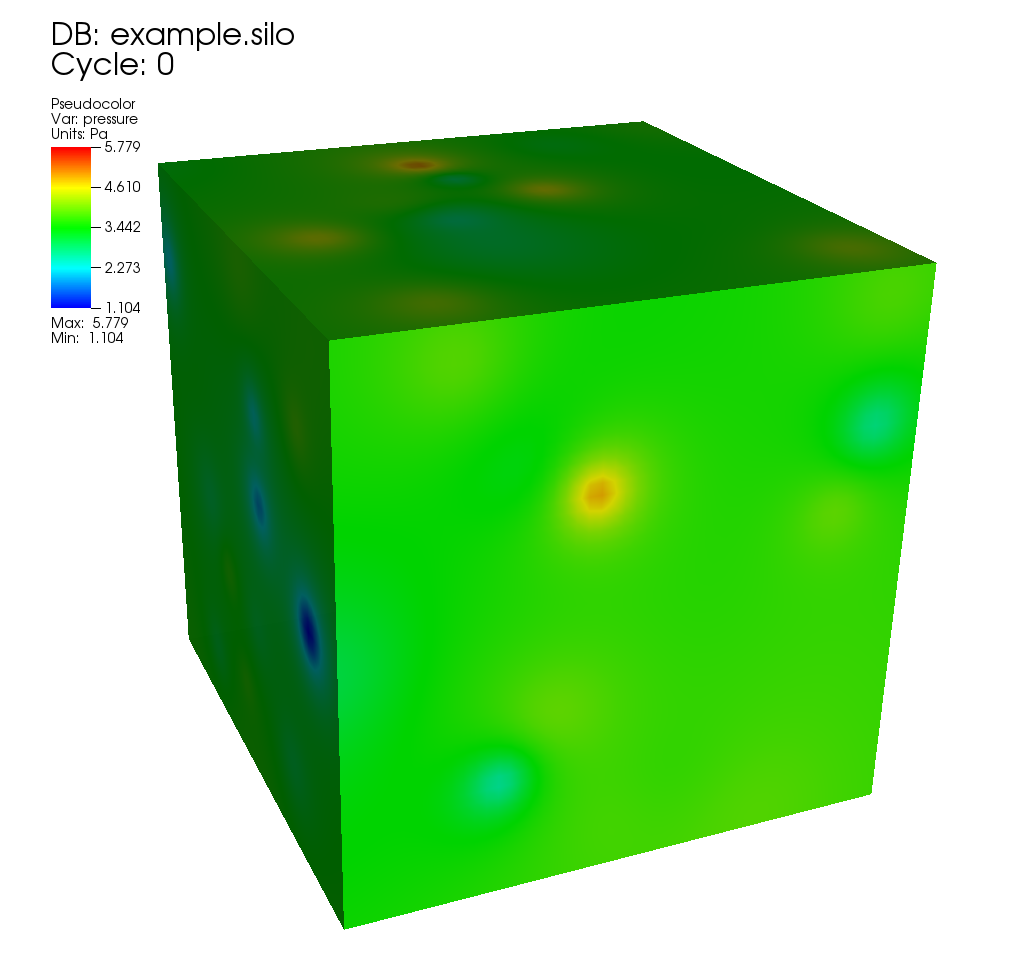
\includegraphics[width=5.8cm]{figs/visit0000.png}
	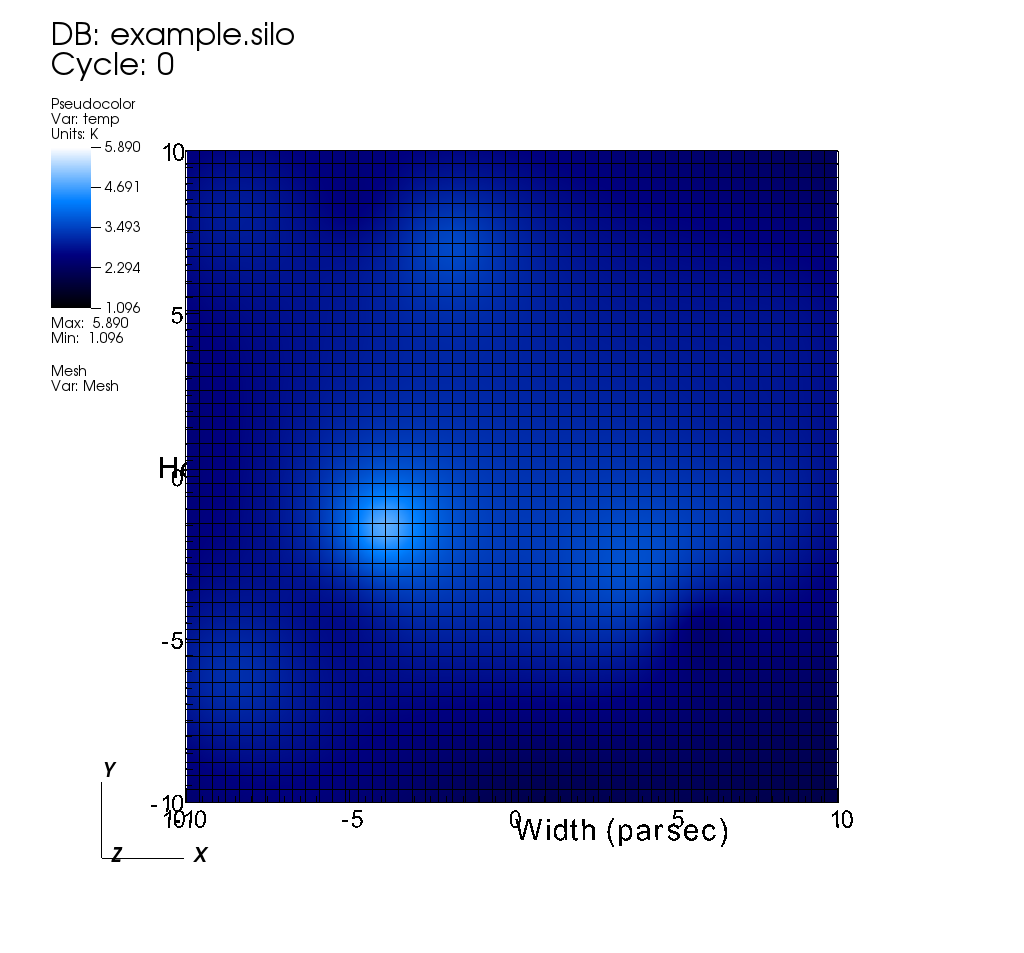
\includegraphics[width=5.8cm]{figs/visit0002.png}
\end{frame}

\begin{frame}{Solución 1}
	\centering
	\includegraphics[width=10cm]{figs/pic4.png}
\end{frame}

\begin{frame}{Solución 2}
	\includegraphics[width=5cm]{figs/pic5.png}
	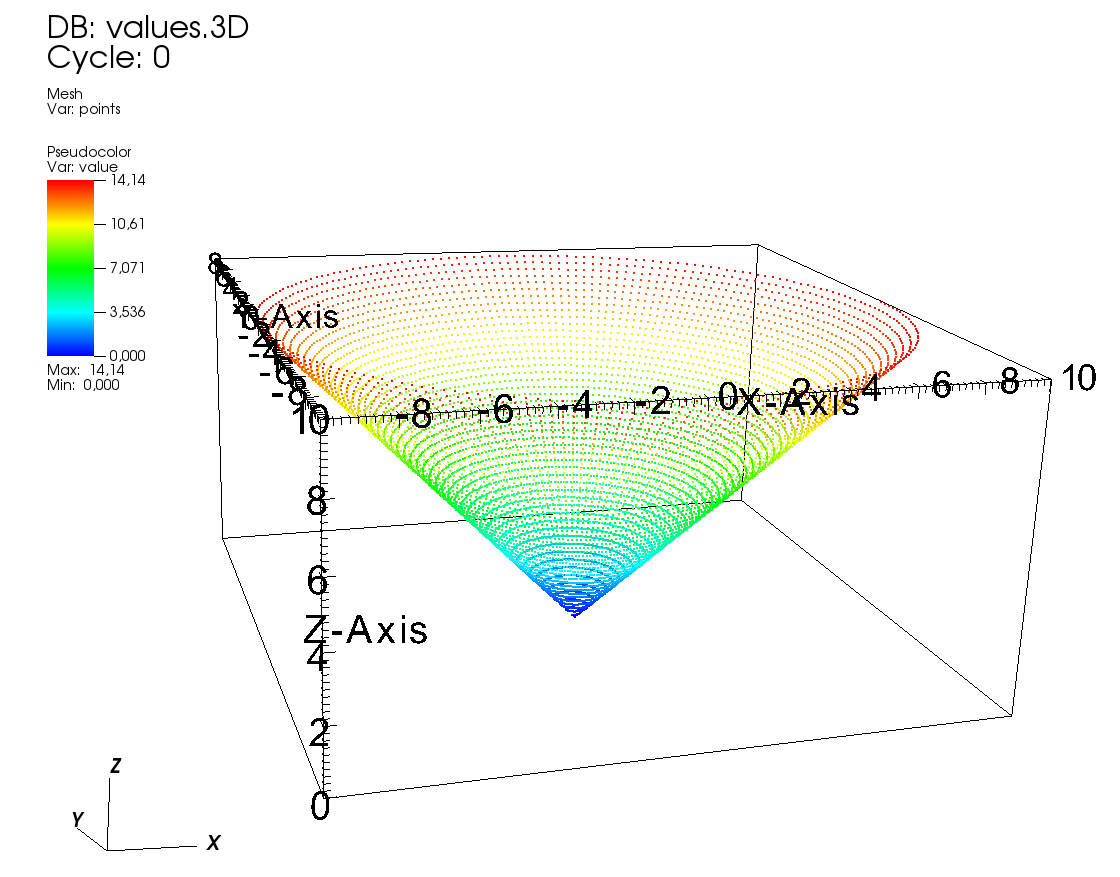
\includegraphics[width=6cm]{figs/visitcreate.png}
\end{frame}

\begin{frame}{}
	\centering
	\includegraphics[width=6.5cm, trim= 0 0 0 0.1cm, clip=true]{figs/pic6.png}
\end{frame}

\begin{frame}{}
	\centering
	\includegraphics[width=11cm]{figs/pic7.png}
\end{frame}

\begin{frame}{}
	\centering
	\includegraphics[width=11cm]{figs/pic8.png}
\end{frame}

\begin{frame}{}
	\centering
	\includegraphics[width=9cm]{figs/pic9.png}
\end{frame}

\begin{frame}{Archivos resultantes}
	\centering
	\includegraphics[width=9cm]{figs/pic10.png}
\end{frame}

\begin{frame}{Script en bash}
	\centering
	\includegraphics[width=9cm]{figs/pic11.png}
\end{frame}

\begin{frame}{}
	\centering
	\includegraphics[width=11cm]{figs/visit1.png}
\end{frame}

\begin{frame}{}
	\centering
	\includegraphics[width=10cm]{figs/visit2.png}
\end{frame}

\begin{frame}{}
	\centering
	\includegraphics[width=10cm]{figs/visit3.png}
\end{frame}

\begin{frame}{}
	\centering
	\includegraphics[width=10cm]{figs/visit4.png}
\end{frame}

\begin{frame}{}
	\centering
	\includegraphics[width=9cm]{figs/rho1.png}
\end{frame}

\begin{frame}{}
	\centering
	\includegraphics[width=8.5cm]{figs/rho2.png}
\end{frame}

\begin{frame}{}
	\centering
	\includegraphics[width=8.5cm]{figs/rho3.png}
\end{frame}

\begin{frame}{}
	\centering
	\includegraphics[width=8.5cm]{figs/rho4.png}
\end{frame}

\begin{frame}{}
	\centering
	\includegraphics[width=8.5cm]{figs/rho5.png}
\end{frame}

\begin{frame}{Referencias}
	\begin{enumerate}
		\item \href{https://wci.llnl.gov/simulation/computer-codes/visit/}{Página oficial de VisIt}
		\item \href{https://github.com/philrosenfield/ascii2hdf5}{Convertidor de ASCII a HDF5}
		\item \href{https://www.visitusers.org/index.php?title=Reading_point_data}{Generador de archivos en formato permitido}
	\end{enumerate}

\end{frame}




%%%%%%%%%%%%%%%%%%%%%%%%%%%%%%%%%%%%%%%%%%%%%%%%%%%%%%%%%%%%%%%%%%

\begin{frame}
\begin{center}
\Huge ¡GRACIAS!
\end{center}
\end{frame}

%%%%%%%%%%%%%%%%%%%%%%%%%%%%%%%%%%%%%%%%%%%%%%%%%%%%%%%%%%%%%%%%%%
\end{document}